%!TEX root = ../MasterThesis.tex

\section{The Semantic Web}
\label{sec:semantic_web}

\subsection{Vision}
\label{sec:semantic_vision}

make information on the Web accessible to machines \\
- allows integration of information across web sites \\
- is also known as the ``Web of Data'' \\
\\
design principles: \\
1. make structured and semi-structured data available in standardized formats \\
2. make individual data elements and their relationships accessible on the Web \\
3. describe the intended semantics of the data in a machine readable format \\
\\
HTML is just for human consumption and a lot of the structures and semantics of the
underlying databases is lost in the transformation process \\
- use labeled graphs as data model for objects and their relationships (objects == nodes,
edges == relationships between them) \\
- formalize the syntax of the graph in RDF (Resource Description Framework) \\
- use URIs to identify individual data items and relations \\
- use ontologies to represent semantics of the data items (either lightweight RDF schema definitions
or Web Ontology Language are used for that) \\
\\
RDFS and OWL are meta-description languages allowing to define new domain-specific knowledge representations \\
they rely on the basic principles of the Web: supporting distributed, decentralized architectures \\
\\
some new initiatives for standardizing semantics: schema.org and linkeddata.org \\
initially it was tried to solve the integration issues with XML, but as it is syntactically more machine-
readable it lacks the semantic of the data \\
- as of this RDF is the basic language of the Semantic Web and describes meta-data as well as content \\
\\
an ontology formally describe a domain based on terms and their relationships (terms == classes of objects) \\
hierarchies are supported (even multiple inheritance between objects) \\
ontologies also include: \\
- properties \\
- value restrictions \\
- disjointness statements \\
- specifications of logical relationships \\
goal is to provide a shared understanding of a domain \\
can help with the necessity to overcome differences in terminology \\
a mapping for different wordings in an ontology or between ontologies is possible \\
they can also be useful for generalization or specialization of Web search results \\
\\
ontologies help with reasoning of objects, they can uncover unexpected relationships and
inconsistencies as well as - by utilizing intelligent web agents - make decisions and select course of actions
(e.g. ``if-then-conclusions'' aka Horn logic) \\
agents can also be used for ``validation of proof'' of statements of another agent or machine \\
\\
Semantic Web is a layered approach \ldots

\begin{figure}[H]
	\centering
		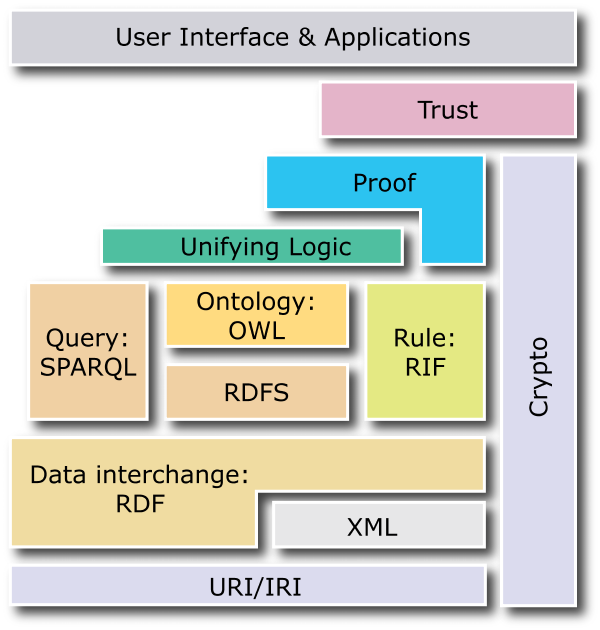
\includegraphics[height=2.5in]{images/semantic_web_layers.png}
	\caption{The Semantic Web Model \citep{W3C2013}}
\label{fig:images_semweb_model}
\end{figure}

% section semantic_vision (end)

\subsection{Resource Description Language}
\label{sec:semantic_rdl}

what is needed to exchange information? \\
1. syntax: how to serialize the data? \\
2. data model: how to structure and organize the data? \\
3. semantics: how to interpret the data? \\
\\
HTML is made for rendering information on screen and for human consumption \\
RDF brings a flexible data model to the Web: \\
- basic building block is a \textbf{triple} of \textit{entity - attribute - value}
also known as statement (could also be expressed as \textit{subject - predicate - object}) \\
RDFS describes the vocabulary that is available \\
\\
so: \\
1. syntax: Turtle, RDFa, RDF-XML or JSON-LD \\
2. data model: RDF \\
3. semantics: RDFS \\
\\
foundational elements are: \\
- resources (aka just a ``thing'' of interest identified by an URI or URL depending on its accessibility) \\
- properties (specify the relations between resources, also identified by URIs) \\
- statements (assign a value to a `resource-property' relation, value could be another resource or a literal) \\
- graphs (RDF is a graph-centered data model, could be distributed, Web of Data / Linked Data approaches) \\
\\
linked data principles: \\
- use URIs as name for things \\
- use HTTP URLs so ppl. can look up those things on the Web \\
- if they do so, provide useful information (HTML and/or RDF, content and/or meta data) \\
- include links to other URLs so they can discover more/related things \\
\\
named graph: \\
- can be used to point to specific statements or (sub-)graphs \\
- alternative: reification via an auxiliary object \\
\\
Turtle: Terse RDF triple language \\
- \textless subject incl. URI \textgreater \textless predicate incl. URI \textgreater \textless object incl. URI \textgreater . \\
- literals will be expressed as ``value''^^\textless XML schema data type \textgreater and supports string, integer, decimal, dates \\
- URIs can be prefixed: @prefix: \textless URI \textgreater \\
- repetition: `;' repeats the subject from previous statement, `,' repeats subject and predicate from previous statement \\

% section semantic_rdl (end)

\subsection{Web Ontologies}
\label{sec:semantic_ontologies}


% section semantic_ontologies (end)

\subsection{Query Language}
\label{sec:semantic_querylang}


% section semantic_querylang (end)

\subsection{Agents and Rules}
\label{sec:semantic_logic_rules}


% section semantic_logic_rules (end)

% section semantic_web (end)
